\cleardoublepage

\lgf{\chapter{ARCHITECTURE POUR L'IOT}}
\lge{\chapter{ARCHITECTURE FOR IOT}}

\section{Introduction}
  
    \vspace{1em}
   
 \begin{wrapfigure}{r}{3cm}
\Youtube{https://youtu.be/DjRhnbg0FjY}
\end{wrapfigure}

\lgf{Les objets se caractérisent par une capacité
de traitement limitée et par une consommation énergétique réduite pour préserver l’autonomie imposée par une alimentation sur batterie.
Or, les activités les plus consommatrices pour un équipement sont l’émission et la réception de données. 
Pour maximiser l’autonomie des équipements, il faut revoir l’intégralité des protocoles, mais en les calquant sur les architectures existantes pour en assurer la compatibilité. 
}
\lge{The objects are characterized by a limited processing capacity and by a reduced energy consumption to preserve the autonomy imposed by a battery power supply.
However, the most consuming activities for an equipment are the transmission and reception of data. 
To maximize the autonomy of equipment, it is necessary to review all the protocols, but by modeling them on existing architectures to ensure compatibility. 
}

\lgf{La figure~\vref{fig-pile-IoT} reprend un certain nombre d'adaptation protocolaires, à différents niveau du modèle \ac{ISO}, capable de s'adapter aux caractéristiques des objets contraints. Dans les chapitres suivants nous reviendrons sur ces technologies en partant de la représentation des données pour aller jusqu'aux couches basses.}
\lge{The figure~\vref{fig-pile-IoT} shows a number of protocol adaptations, at different layers of the model, capable of adapting to the characteristics of the constrained objects. In the following chapters, we will come back to these technologies, starting from the data representation and going to the lower layers.}

\begin{figure}[tbp]
\centerline{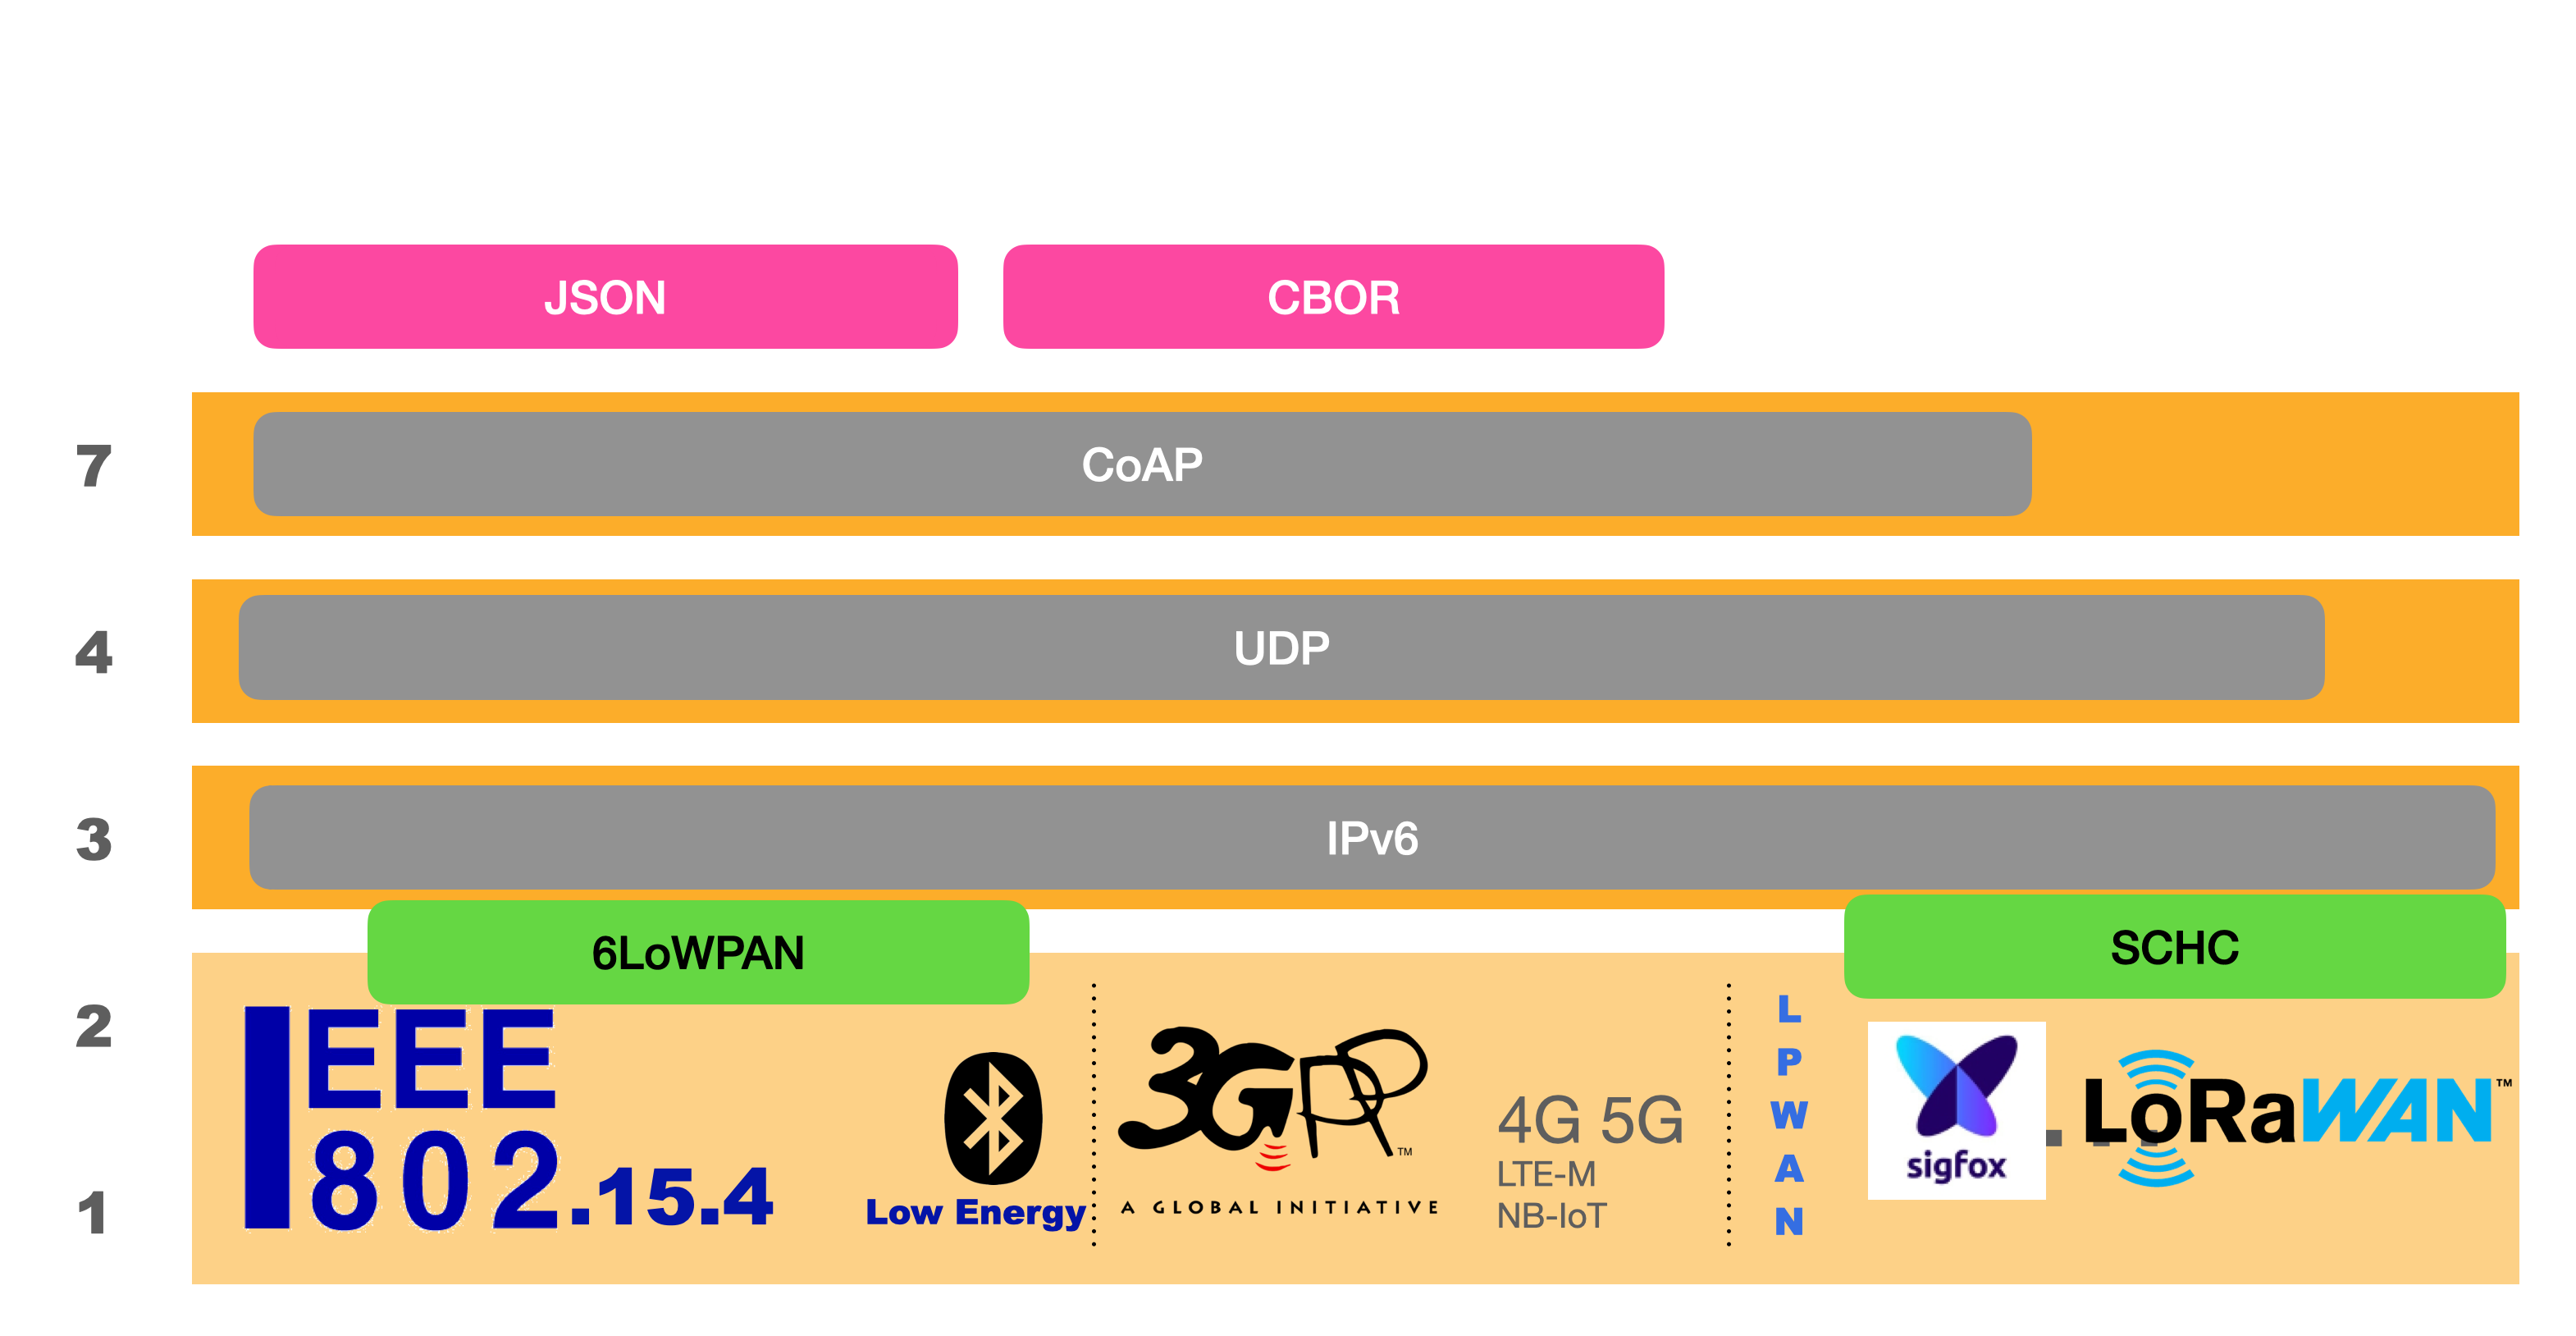
\includegraphics[width=1\columnwidth]{Pictures/Capture17.png}}
\lgf{\caption{Pile protocolaire de l'IoT}}
\lge{\caption{IoT protocol stack}}
\label{fig-pile-IoT}
\end{figure}

\lgf{\section{Topologies}}
\lge{\section{Topologies}}

\lgf{Les réseaux pour l’internet des objets peuvent être divisés en deux catégories : les topologies \Index{maillé}es (\Index{Mesh} in english) et étoilées (\Index{star}).}
\lge{Networks for the Internet of Things can be divided into two categories: \Index{mesh} and \Index{star} topologies.}

\lgf{\subsection*{Réseaux Maillés}}
\lge{\subsection*{Mesh Networks}}

\lgf{Les réseaux maillés, tels que la famille IEEE 802.15.4,  sont une adaptation d’un protocole d’accès Wi-Fi pour préserver l’énergie. La portée de transmission est limitée à 50 mètres pour limiter la consommation d'énergie ; et par conséquent les messages doivent être relayés par d’autres nœuds pour atteindre leur destination.}
\lge{Mesh networks, such as the IEEE 802.15.4 family, are an adaptation of a Wi-Fi access protocol to preserve energy. The transmission range is limited to 50 meters to limit energy consumption, and therefore messages must be relayed by other nodes to reach their destination.}

\lgf{Le débit est de quelques centaines de kilobits/s et la taille de la trame est de quelques centaines d’octets. }
\lge{The data rate is a few hundred kilobits/s and the frame size is a few hundred bytes. }

\lgf{Ces réseaux sont performants pour transporter des données IoT, mais le protocole de routage, ainsi que le relayage des trames, consomment l’énergie des objets.}
\lge{These networks are good at carrying IoT data, but the routing protocol, as well as frame relaying, consumes the objects' energy.}

\lgf{\subsection*{Réseaux en Étoile}}\lge{\subsection*{Star Network}}\label{chap-star}

\lgf{Les topologies en \Index{étoile} ne nécessitent pas de tels mécanismes de routage. Toutes les communications se font avec un point central qui relaie les informations vers la destination.}
\lge{The topologies in \Index{star} do not require such routing mechanisms. All communications are with a central point that relays information to the destination.}

\lgf{Les progrès réalisés dans le traitement des signaux permettent d’étendre la portée de transmission à faible puissance. Cette famille de réseaux est appelée réseaux étendus à faible puissance (\ac{LPWAN}) comme \Index{Sigfox}, \Index{LoRaWAN}, ou même du côté de la téléphonie cellulaire avec des évolutions de la norme \Index{4G} et une intégration plus complète dans la \Index{5G}. Le \rfc{8376} donne, en anglais, un aperçu de ces techniques.}
\lge{The progress made in signal processing allows to extend the transmission range at low power. This family of networks is called low power wide area networks (LPWAN) like \Index{Sigfox}, \Index{LoRaWAN}, or even on the cellular side with evolutions of the \Index{4G} standard and a more complete integration in \Index{5G}. The \rfc{8376} gives, in English, an overview of these techniques.}


    \vspace{1em}

\lgf{Avec une puissance de transmission de 25 mW, il est possible de communiquer sur une distance de 3 km en milieu urbain et de 20 km dans un environnement dégagé. Les \ac{LPWAN} sont compatibles avec les appareils de classe 0 car ils ne nécessitent pas la mise en place d’une pile \ac{IP}. La figure ci-dessous décrit une architecture typique pour les \ac{LPWAN}.}
\lge{With a transmission power of 25 mW, it is possible to communicate over a distance of 3 km in an urban environment and 20 km in a clear environment. The LPWANs are compatible with class 0 devices because they do not require the installation of an IP stack. The figure below describes a typical architecture for LPWANs.}

\begin{figure}[tbp]
\centerline{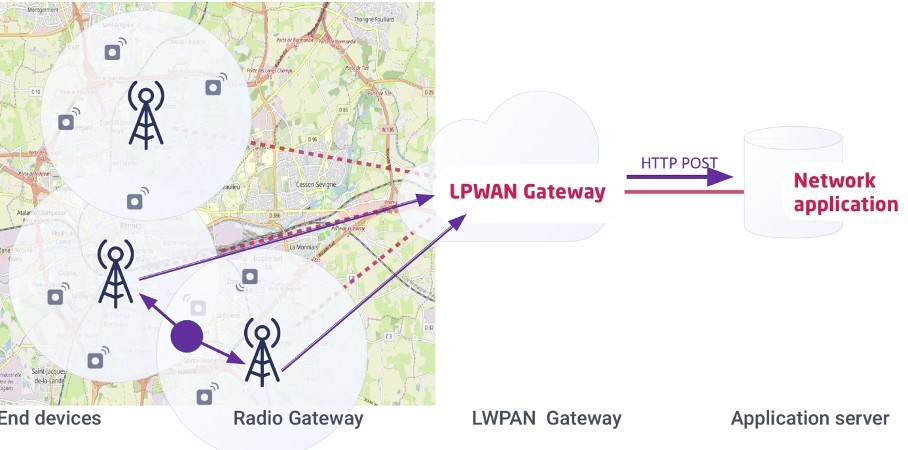
\includegraphics[width=1\columnwidth]{Pictures/TolologieStar.jpg}}
\lgf{\caption{Architecture simplifiée des réseaux LPWAN}}
\lge{\caption{Simplified LPWAN architecture}}
\label{fig-topo-star}
\end{figure}


\lgf{L’appareil envoie des données brutes sur le réseau radio. Le signal radio est capté par une ou plusieurs passerelles radio, et la trame est envoyée à une passerelle réseau (\ac{LNS}  pour les réseaux \Index{LoRaWAN}, et \ac{SCEF} pour les réseaux \ac{3GPP}).}
\lge{The device sends raw data over the radio network. The radio signal is picked up by one or more radio gateways, and the frame is sent to a network gateway (\ac{LNS} for networks \Index{LoRaWAN}, and \ac{SCEF} for networks \ac{3GPP}).}

\lgf{Le propriétaire de l’appareil a associé l’appareil à un connecteur dans le LPWAN \ac{NGW} qui peut être un \ac{URI}, une adresse de broker \ac{MQTT} ou une Web socket. Lorsque l’appareil envoie des données, il est relié à l’application par ce tunnel.}
\lge{The owner of the device has associated the device with a connector in the LPWAN \ac{NGW} which can be a URL, a \ac{MQTT} broker  address or a web socket. When the device sends data, it is connected to the application through this tunnel.}

    \vspace{1em}


\lgf{Certaines technologies telles que LoRaWAN ou Sigfox utilisent des bandes sans licence, imposant un cycle d’utilisation (\Index{Duty Cycle}) de 0,1 à 10 \% selon les canaux pour assurer l’équité entre les nœuds, empêchant ainsi qu'un équipement ne monopolise le canal de transmission. Comme cette restriction s’applique également à l’antenne du fournisseur, la communication entre le réseau et l’appareil est considérablement limitée.}
\lge{Some technologies such as LoRaWAN or Sigfox use unlicensed bands, imposing a duty cycle of 0.1 to 10 percent depending on the channel to ensure fairness between nodes, thus preventing one device from monopolizing the transmission channel. Since this restriction also applies to the provider's antenna, communication between the network and the device is significantly limited.}

\lgf{L’utilisation principale de ces réseaux \ac{LPWAN} est la télémétrie où un appareil envoie régulièrement des informations ou une alarme de temps en temps (par exemple des capteurs de température). Le débit et la taille des messages est beaucoup plus réduit que dans le cas de réseaux maillés.}
\lgf{The main use of these \ac{LPWAN} networks is telemetry where a device regularly sends information or an alarm from time to time (for example temperature sensors). The throughput and the size of the messages is much smaller than in the case of mesh networks.}

    \vspace{1em}

\lgf{\section{Niveaux 1 et 2}}
\lge{\section{Layers 1 and 2}}

 \lgf{Concernant le niveau 2, le but est de gagner en énergie lors des transmissions. Déjà on peut dire adieu à Ethernet car cela imposerait d'utiliser l'infrastructure filaire et donc on ne pourrait pas placer les objets où on veut, surtout s'ils se déplacent. Les communications par ondes radio sont privilégiées. }
 \lge{Concerning layer 2, the goal is to save energy during transmissions. We can already say goodbye to Ethernet because it would require the use of wired infrastructure and therefore we could not place the objects where we want, especially if they move. The communications by radio waves are privileged. }
 
 \lgf{Pour l'Internet des objets, le \Index{Wi-Fi} est également trop gourmand en énergie. On lui préfère donc une évolution appelée \Index{IEEE 802.15.4} qui reprend son principe de fonctionnement mais l'adapte à un faible débit et à des trames de petite taille. En particulier pour économiser l'énergie, la portée est réduite à une dizaine de mètres et il faut généralement utiliser des relais pour atteindre une destination. }
 \lge{For the Internet of Things, Wi-Fi is also too power-hungry. It is therefore preferred to an evolution called \Index{IEEE 802.15.4} which uses its operating principle but adapts it to a low speed and to small frames. In particular to save energy, the range is reduced to about ten meters and it is generally necessary to use relays to reach a destination. }
 
\lgf{\Index{Bluetooth} a été adapté pour des objets avec une basse consommation \ac{BLE}. }
\lge{\Index{Bluetooth} has been adapted for objects with a low consumption \ac{BLE}. }
     \vspace{1em}

 \lgf{Côté téléphonie cellulaire, les protocoles évoluent pour prendre en compte les objets. La norme 4G a intégrée les communications à plus bas débit. La 5G inclura une classe permettant des communications avec les objets économes en énergie et réduisant les temps de latence. }
 \lge{On the cellular side, protocols are evolving to take objects into account. The 4G standard has integrated lower speed communications. The 5G will include a class allowing communications with objects energy efficient and reducing latency. }
 
\lgf{\section{IP et couches d'adaptation}}
\lge{\section{IP and adaptation layers}}

\lgf{At layer 3, we go towards the more massive use of \ac{IPv6} since version 4 has its address space saturated. The size of the address is extended on 128 bits offering $2^{96}$ times more addresses.}
  
  \begin{figure}[tbp]
\centerline{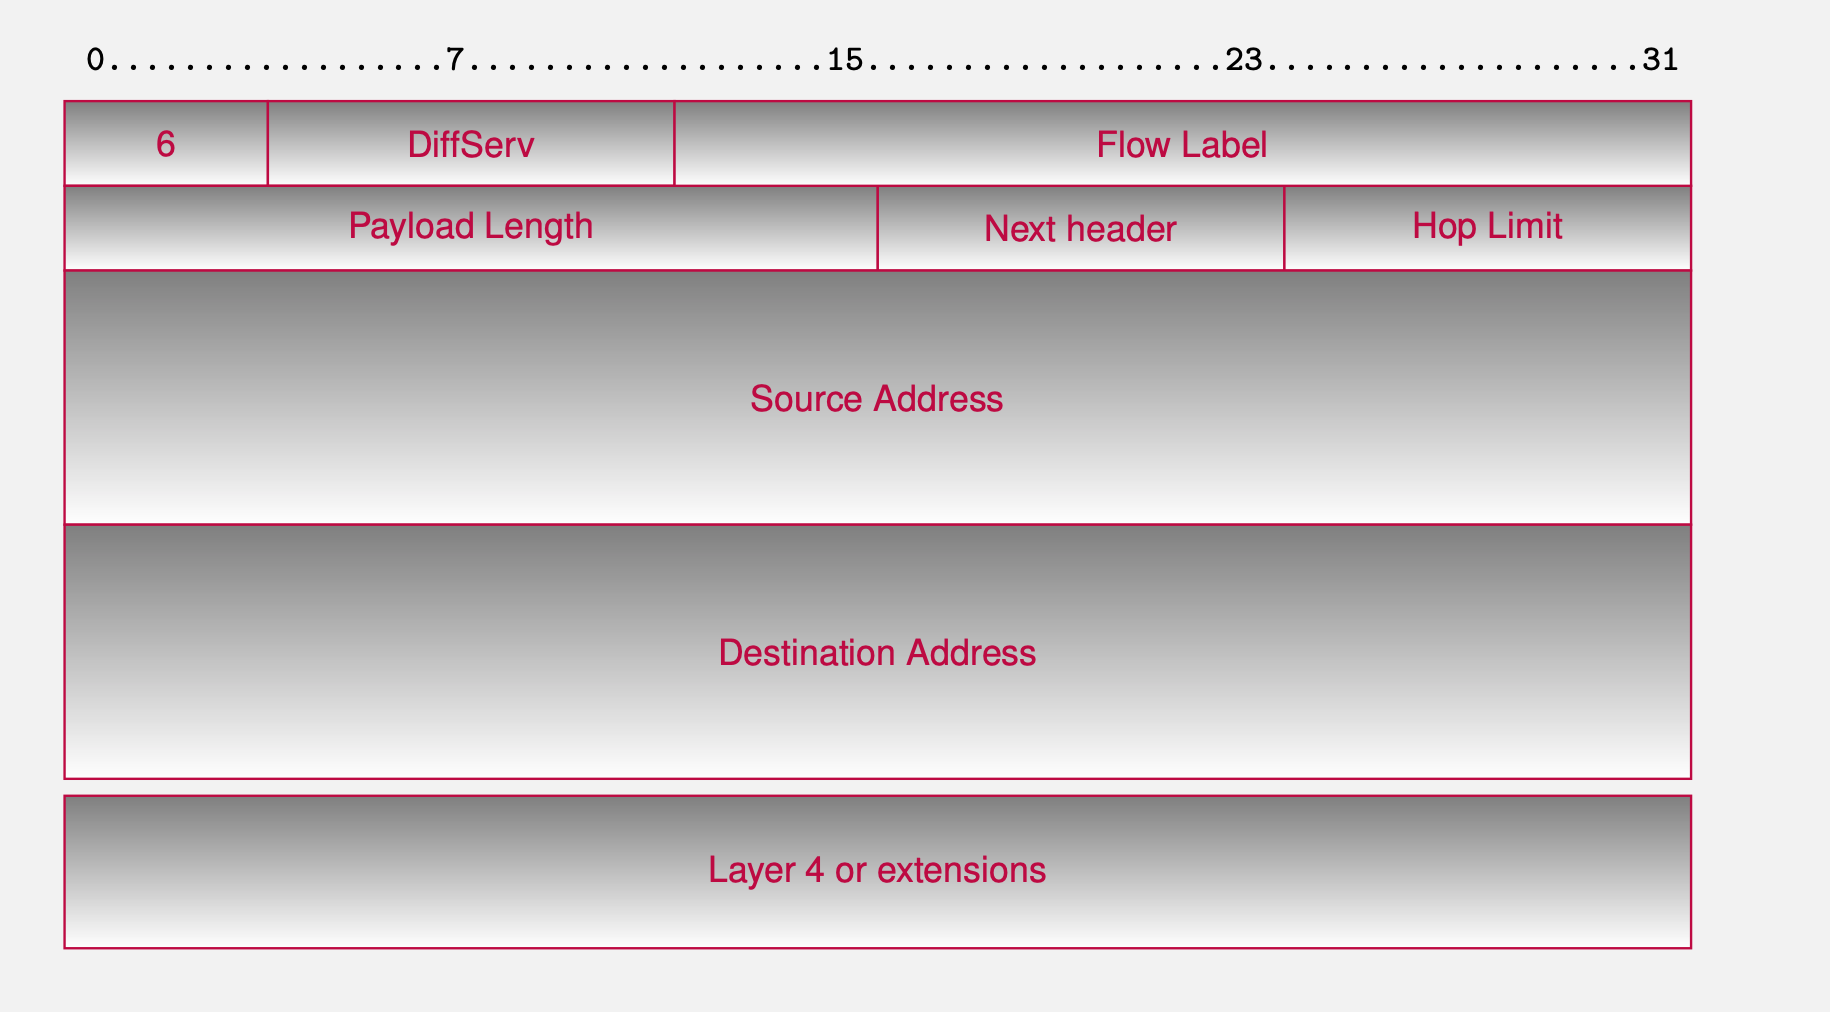
\includegraphics[width=1\columnwidth]{Pictures/Capture18.png}}
\lgf{\caption{Format d'un en-tête IPv6}}
\lge{\caption{IPv6 header format}}
\label{fig-IPv6-header}
\end{figure}
  
\lgf{Mais, comme on le voir sur la figure~\vref{fig-IPv6-header} \ac{IPv6} implique des en-têtes plus grandes, ce qui est gênant car les réseaux de niveau 2 transportent de plus petites trames.
Une \Index{couche d'adaptation} entre la couche \ac{IP} et le niveau 2 est nécessaire puisque les niveaux 2 conçus pour l'internet des objets ne peuvent pas transporter naturellement de grands paquets. Deux actions sont mises en œuvre : \Index{compression} de la taille des en-têtes pour réduire leur impact, et \Index{fragmentation} pour découper le paquet en petites trames si la première mesure ne suffit pas. }
\lge{But, as seen in Figure~\vref{fig-IPv6-header} \ac{IPv6} implies larger headers, which is troublesome because Layer 2 networks carry smaller frames.
An \Index{adaptation layer} between the \ac{IP} layer and Layer 2 is needed since Layer 2s designed for the Internet of Things cannot naturally carry large packets. Two actions are implemented: \Index{compression} of header size to reduce their impact, and \Index{fragmentation} to break the packet into smaller frames if the first measure is not sufficient. }

     \vspace{1em}

\lgf{Il existe deux grandes familles de couche d'adaptation :}
\lge{There are two main families of adaptive layers:}

\begin{itemize}
    \item 
        \lgf{\Index{6LoWPAN} \rfc{4944}, \rfc{6282}, qui va intégrer un mécanisme de compression de l'en-tête \ac{IPv6} et de fragmentation pour envoyer un gros paquet divisé en petites trames. En effet, dans un réseau maillé, il n'est pas possible de se priver d'informations fournies par la couche \ac{IP} car les nœuds intermédiaires en ont besoin pour acheminer le message vers le destinataire. 6LoWPAN est sans état et compresse toutes les en-têtes IPv6 sans configuration. }
        \lge{\Index{6LoWPAN} \rfc{4944}, \rfc{6282}, which will integrate a mechanism of compression of the header \ac{IPv6} and of fragmentation to send a large packet divided into small frames. Indeed, in a mesh network, it is not possible to deprive oneself of information provided by the IP layer because the intermediate nodes need it to route the message to the recipient. 6LoWPAN is stateless and compresses all IPv6 headers without configuration. }

    \item 
        \lgf{\ac{SCHC} (prononcer chic) \rfc{8724} va imposer des règles décrivant l'en-tête du message et va envoyer le numéro de la règle en remplacement de l'en-tête. La compression est beaucoup plus importante et peut porter sur plusieurs couches protocolaires. Cependant, pour la mettre en œuvre, il faut avoir une idée des flux qui vont circuler sur le réseau. \ac{SCHC} est spécifié pour les réseaux en \Index{étoile} et plus particulièrement les \ac{LPWAN}.}
        \lge{\ac{SCHC} (pronounce chic) \rfc{8724} will impose rules describing the message header and will send the rule number in place of the header. Compression is much more important and can involve several protocol layers. However, to implement it, you need to have an idea of the flows that will circulate on the network. \ac{SCHC} is specified for networks in \Index{star} and more particularly for \ac{LPWANs}.}

\end{itemize}

\lgf{\section{Mise en \oe{}uvre de \Index{REST}}}
\lge{\section{Implementation of \Index{REST}}}
  
\lgf{Au-dessus on avait vu que comme \ac{HTTP} était le protocole dominant, \ac{TCP} l'était aussi. Mais pour l'IoT ce n'est pas optimal. En effet TCP/HTTP sont des protocoles complexes qui demandent beaucoup de mémoire. Pour réduire l'impact de la pile protocolaire, l'\ac{IETF} a défini un nouveau protocole appelé \ac{CoAP} qui demande que quelques Kilo Octets pour fonctionner. \ac{CoAP} repose sur \ac{UDP} ce qui simplifie encore la mise en oeuvre. }
\lge{Above we had seen that as \ac{HTTP} was the dominant protocol, \ac{TCP} was also. But for the IoT this is not optimal. Indeed TCP/HTTP are complex protocols that require a lot of memory. To reduce the impact of the protocol stack, the IETF has defined a new protocol called CoAP which requires only a few Kilobytes to work. \ac{CoAP} is based on UDP which simplifies again the implementation. }
  
  
       \vspace{1em}

\lgf{Pour poursuivre dans l’intégration des objets dans l’internet, le protocole \ac{CoAP} \rfc{7252} se substitue à \ac{HTTP}. Il en reprend le mécanisme de nommage, d’utilisation des ressources, et les primitives de manipulation entre un client et un serveur.}
\lge{To continue in the integration of the objects in the Internet, the protocol \ac{CoAP} \rfc{7252} replaces \ac{HTTP}. It takes over the naming mechanism, the use of resources, and the handling primitives between a client and a server.}

\lgf{La capacité de traitement du capteur et son alimentation  en énergie sont souvent très limitées. 
La grande force de \ac{CoAP} est d’être :}
\lge{The processing capacity of the sensor and its power supply are often very limited. 
The great strength of \ac{CoAP} is to be:}

\begin{itemize}
\item 
    \lgf{facile à mettre en œuvre. Les mises en œuvre de \ac{CoAP} nécessitent peu de mémoire ;}
    \lge{easy to implement. The implementations of \ac{CoAP} require little memory;}
\item 
    \lgf{fully compatible with \ac{HTTP} and it is possible to go from one 
protocol to the other through generic gateways, i.e. not linked 
to a particular use (as shown in figure~\vref{fig-encap}).}
\end{itemize}

\lgf{De ce fait, \ac{CoAP} va manipuler des ressources, identifiées par des \ac{URI}. Il est donc possible d'ancrer les données fournies par les objets dans l'écosystème actuel des communications entre ordinateurs, fortement structuré autour des principes REST.}
\lge{As a result, CoAP will manipulate resources, identified by \ac{URI}s. It is thus possible to anchor the data provided by the objects in the current ecosystem of communications between computers, strongly structured around the REST principles.}

     \vspace{1em}

\lgf{La sécurité, en particulier le chiffrement des données, suit aussi les mêmes chemins que l’internet traditionnel.  Il existe un chiffrement au-dessus d’\ac{UDP} qui, à l’instar de \ac{HTTPS}, chiffre les échanges.}
\lge{Security, especially data encryption, also follows the same paths as the traditional Internet.  There is an encryption above \ac{UDP} which, like \ac{HTTPS}, encrypts the exchanges.}
  
\lgf{\section{Représentation des données}}
\lge{\section{Data representation}}

\lgf{Pour la structuration des données, \ac{XML} n'est pas utilisée car il est trop bavard. \ac{JSON} est beaucoup plus efficace pour transporter des informations structurées. Il existe un équivalent binaire que nous verrons par la suite \ac{CBOR} qui est beaucoup plus performant, et simple à mettre en oeuvre est compatible avec JSON.}
\lge{For data structuring, XML is not used because it is too talkative. \ac{JSON} is much more effective to transport structured information. There is a binary equivalent that we will see later : CBOR, which is much more efficient, and simple to implement, and compatible with JSON.}

\lgf{\section {Alternatives à REST}}
\lge{\section {Alternatives to REST}}


\lgf{Il n'est pas obligé de tout mettre en oeuvre tous les protocoles définis par l'IETF. Il est possible également d'y intégrer des protocoles spécifiés pour un métier. }
\lge{It does not have to implement all the protocols defined by the IETF. It is also possible to integrate protocols specified for a business. }

   \begin{wrapfigure}{r}{7cm}
\centerline{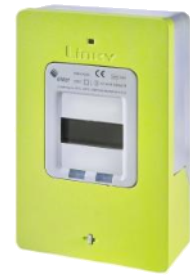
\includegraphics[width=.4\columnwidth]{Pictures/linky.png}}
\end{wrapfigure}

\lgf{Par exemple, le compteur électrique \Index{Linky} que tous les Français connaissent en implémente qu'une partie. Au lieu d'utiliser \ac{CoAP}, les électriciens utilisent leurs propres applications suivant la norme \ac{DLMS}/\ac{Cosem}. Celle-ci repose sur \ac{UDP} puis \ac{IPv6} et \Index{6LoWPAN} et finalement sur une variante de \Index{IEEE 802.15.4} adaptée pour transporter l'information sur les câbles électriques.}
\lge{For example, the electric meter \Index{Linky} that all French people know implements only a part of it. Instead of using CoAP, the electricians use their own applications following the standard DLMS/Cosem. This one is based on \ac{UDP} then \ac{IPv6} and \Index{6LoWPAN} and finally on a variant of \Index{IEEE 802.15.4} adapted to transport the information on the electric cables.}

